Kolejną propozycją jest link radiowy. Są to rozwiązania niewiele tańsze oraz mniej skomplikowane. Wydają się być w zupełności wystarczające na potrzeby projektu. Podczas planowania przedstawione zostały następujące warianty:

\begin{itemize}
\item Gotowy moduł od Texas Instruments z serii CC11xx
\item Użycie kart sieciowych 
\item Stworzenie własnych modułów komunikacji radiowej
\end{itemize}

Już na początku można zauważyć, że tworzenie własnego modułu jest bardzo czasochłonne oraz wymaga pisania od nowa wszystkich sterowników. Rezultaty też nigdy nie będą takie jak w przypadku droższych, komercyjnych rozwiązań.

Do zalet gotowego modułu od Texas Instruments należą:

\begin{itemize}
\item częstotliwości 169,433,868,915,920 MHz
\item niski pobór prądu
\item wzmacniacz np. CC1190 (+0,5W)
\item programowalna moc wyjściowa
\item modulacje 2-FSK,2-GFSK,4-FSK,4-GFSK,OOK
\item Wake-On-Radio
\item single-chip
\end{itemize}

Wadą natomiast jest bardzo mała przepustowość (1.25 Mbps).

\begin{figure}[H]
\centering
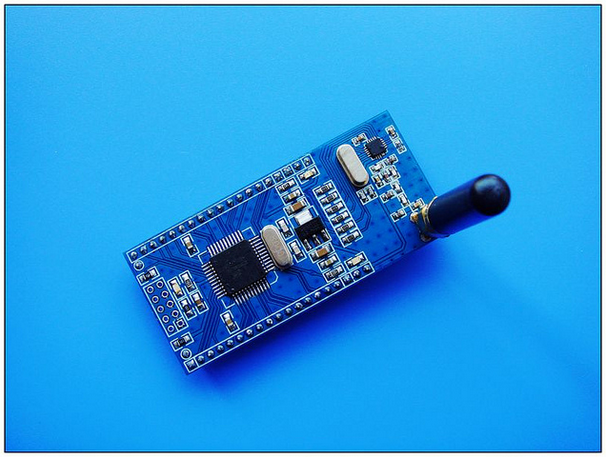
\includegraphics[width=0.7\textwidth]{./grafika/link.png}
\caption[Moduł radiowy TI CC1200]}
\end{figure}

Łatwiej dostępnym i bardziej sprawdzonym rozwiązaniem jest wykorzystanie wszechobecnych kart sieciowych.

Do zalet takiego rozwiązania można zaliczyć:

\begin{itemize}
\item Łatwy dostęp i duży wybór gotowych rozwiązań
\item Sterowniki oraz aplikacja obsługująca urządzenie w wybranym
\item środowisko nie jest problemem
\item Prędkość transmisji
\end{itemize}

Wady:

\begin{itemize}
\item Praca na bardzo wysokich częstotliwościach - możliwe problemy z zasięgiem
\item Podatność na zakłócenia
\item Słabe zabezpieczenia 
\end{itemize}

Pomimo podanych powyżej wad, wydaje się to być najbardziej optymalnym rozwiązaniem, który znalazło zastosowanie w projekcie.